\documentclass[10pt]{article}

% amsmath package, useful for mathematical formulas
\usepackage{amsmath}
% amssymb package, useful for mathematical symbols
\usepackage{amssymb}

% graphicx package, useful for including eps and pdf graphics
% include graphics with the command \includegraphics
\usepackage{graphicx}

% cite package, to clean up citations in the main text. Do not remove.
\usepackage{cite}

\usepackage{color} 

% Use doublespacing - comment out for single spacing
\usepackage{setspace} 
\doublespacing

% Text layout
\topmargin 0.0cm
\oddsidemargin 0.5cm
\evensidemargin 0.5cm
\textwidth 16cm 
\textheight 21cm

% Bold the 'Figure #' in the caption and separate it with a period
% Captions will be left justified
\usepackage[labelfont=bf,labelsep=period,justification=raggedright]{caption}

% Use the PLoS provided bibtex style
\bibliographystyle{plos2009}

% Remove brackets from numbering in List of References
\makeatletter
\renewcommand{\@biblabel}[1]{\quad#1.}
\makeatother


% Leave date blank
\date{}

\pagestyle{myheadings}
%% ** EDIT HERE **


%% ** EDIT HERE **
%% PLEASE INCLUDE ALL MACROS BELOW

\usepackage{multirow}
\renewcommand{\arraystretch}{1.1}

% figure files reside in the figures/ directory
\graphicspath{
{figures/}
}

%% END MACROS SECTION

\begin{document}

% Title must be 150 characters or less
\begin{flushleft}
{\Large
\textbf{Spatially explicit model of the lymphocyte diaspora in influenza-infected lung reveals thresholds on chemokine directed migration}
}
% Insert Author names, affiliations and corresponding author email.
\\
Drew Levin$^{1,\ast}$, 
Stephanie Forrest$^{1}$, 
Soumya Banerjee$^{1}$,
Candice Clay$^{2}$, 
Melanie Moses$^{1}$, 
Frederick Koster$^{1,2}$
\\
\bf{1} Department of Computer Science, University of New Mexico, Albuquerque, NM, USA
\\
\bf{2} Lovelace Respiratory Research Institute, Albuquerque, NM, USA
\\
$\ast$ E-mail: Corresponding drew@cs.unm.edu
\end{flushleft}



% Please keep the abstract between 250 and 300 words
\section*{Abstract}

During the primary immune response, clearance of influenza in the lung requires the homing of activated CD8 T cells from regional lymph nodes to infected foci comprising a fraction of the total lung.  T cell navigation to infected foci is undirected but emigration into tissue is directed by local cytokine and chemokine production from infected epithelial cells.  We focused on the efficiency of local chemokines to induce migration of activated CD8 T cells using a spatially explicit agent-based model (ABM) without constructing a model containing all elements of the immune response.  

To determine local chemokine production, avian H5N1, seasonal H1N1, and 2009 pandemic influenza strains were used \textit{in vitro} to induce the secretion of CXCL10 (IP-10) and CCL5 (RANTES) in human bronchial epithelial cells.  A differential equation model was fit to empirical chemokine production rates and coupled with published T cell parameters to calibrate the spatial model to test inter-strain variation on T cell recruitment in the lungs.  The modeled immune response is unable to clear the pandemic strain due to its high rate of viral production.  

The spatial nature of the ABM model reveals unique challenges to T cell recruitment not appreciated in standard differential equation models.  Infected cells can become isolated in expanding plaques, impeding T cell search, even though the T cells could directionally migrate to low levels of chemokine.  A key limitation imposed on T cells is illustrated by their failure to clear the pandemic H1N1 virus after day 6, when T cells became inefficient in large infected foci. This spatially explicit model is consistent with efficient T cell recruitment to small infected foci in the lung, but as foci become large T cell search becomes inefficient, thus emphasizing the importance of enhanced control early in infection.


% Please keep the Author Summary between 150 and 200 words
% Use first person. PLoS ONE authors please skip this step. 
% Author Summary not valid for PLoS ONE submissions.   
\section*{Author Summary}

Clearance of influenza from the lung depends strongly on the efficiency with which T cells travel from the lymph node to the site of infection.  However, T cells in the lung must navigate the large branching bronchial network.  This maze-like structure is a challenge for T cell search, and the vast majority of T cells exit the lung without encountering infection.  Infected cells produce cytokines and chemokines, which signal T cells to exit the vasculature and enter tissue.  We developed an agent-based model to quantify how these molecular signals affect search.  Our experimental data show that two chemokines, IP-10 and RANTES, are important for T cell search.  We incorporated the data in our spatially explicit model, which allowed us to identify challenges to the search process not obvious in conventional differential equation models.  We ran three sets of simulations, using parameters from seasonal influenza, avian influenza, and 2009 pandemic influenza.  The simulated immune response contains the first two infections but is unable to contain the highly virulent pandemic strain due to the rapidly expanding plaque size.  Direct interventions to improve this T cell search process are unlikely to be effective, and therefore vaccination is required to contain more virulent strains.

\section*{Introduction}

The adaptive immune response induced during acute influenza A infection is a complex combination of defense mechanisms.  Understanding the behavior and interactions of each cellular component may lead to improved vaccines and strategies to control immunopathology.   The innate immune response is critical for early control of viral replication, followed by antibody-mediated viral neutralization \cite{Kohlmeier2009a, Joo2008, Oslund2011}.   Complete resolution of influenza pneumonia depends on antigen-specific CD8+ T effector cells \cite{Cerwenka1999, Kim2011}.  The murine model has been critical in the reductive analysis of each phase and component, permitting temporally explicit descriptions of the induction phase in the regional lymph node \cite{Miller2003, Allan2006, Ingulli2009} where recruitment of clonal precursor CD8 T cells is highly efficient \cite{VanHeijst2009}.   On approximately day 5 after infection, activated CD8 T cells are released from the secondary lymphoid tissue \cite{Miao2010a} and distributed throughout the body in a process known as the ‘lymphocyte diaspora’ \cite{Marshall2001}.

The process of recruitment of activated CD8 effector cells to infected sites in the lung is not completely understood.  Initial localization and extravasation may depend on a number of inflammatory signals but viral antigen does not appear to induce recruitment into tissue \cite{Topham2001}.   Effector cells must localize to sites of viral replication [4], but it is not clear whether cells passing through uninfected lung tissue leave through the pulmonary vein or exit the capillary bed and leave the lung through lymphatic channels. Chemotactic proteins play a major role in recruitment in both acute infections and chronic inflammatory diseases \cite{Bromley2008, Medoff2005} where recruited T cells mediate either protection or immunopathology.  Infected epithelial cells secrete chemokines \cite{Chan2005} and contact with CD8 T cells also triggers secretion \cite{Zhao2000}. Activated CD8 T effector cells upregulate chemotactic protein receptors, particularly CXCR3 and CCR5 \cite{Hoji2005, Groom2011a}, responding to their primary ligands CXCL10 (IP-10) and CCL5 (RANTES) respectively.  

The consequences of chemotactic ligand-receptor interactions, however, are complex \cite{Groom2011a, Groom2011} and variable in the models studied.   For example, in the lymphochoriomeningitis virus model the CXCR3 receptor mediates T cell recruitment to infected brain and subsequent immunopathology \cite{Christensen2004, Christensen2006}, while the CCR5 mediates the opposite effect \cite{DeLemos2005}.  In contrast, in the West Nile virus model \cite{Klein2005} and the dengue model \cite{Hsieh2006}, deficiency of IP-10 reduced T cell recruitment to the brain resulting in higher viral burden and increased mortality.   In the herpesvirus model, IP-10 was critical in T cell recruitment and disease control in the HSV-2-infected brain \cite{Wuest2008, Thapa2008}.  In the parainfluenza virus model, CXCR3 receptor is critical in CD4+ T cell migration to the lung \cite{Kohlmeier2009}.  In the influenza A model, initial studies with chemokine receptor knock-out mice obtained mixed results with respect to changing the course of disease \cite{Dawson2000, Wareing2004}, concluding that redundancy in chemokine signals may confound interpretation.   The CXCR3 receptor mediated T cell localization and spared the increased mortality of CCR5 deficiency, but viral clearance was not altered \cite{Fadel2008}.  The CXCR3 receptor also mediates the balance between effector versus memory cell differentiation among recruited CD8 T cells in the lung \cite{Kohlmeier2011}.   

Although leukocytes exhibit directional behavior to chemokines \cite{LiJeon2002, McDonald2010}, CD8 T cells have not yet been shown to climb chemokine gradients.   Following arrival at the infected site, CD8 T cells secrete cytokines when mononuclear cells are present but in their absence kill infected epithelial cells only by contact cytolysis \cite{Hufford2011}.   Finally the exit of T cells from tissue is tightly regulated to keep effector cells from leaving or dying prematurely \cite{Jennrich2012, Richter2007} but effective life-span is unknown. 

There are many mathematical models of the entire adaptive response \cite{Miao2010, Saenz2010, Beltman2007, Handel2008, Zheng2008, Lee2009}, filling gaps with reasonable assumptions of cellular behavior in the absence of experimental support.  Mathematical and computational models can examine each event in detail and narrow the range of possible behaviors.  Here we examine the CD8 T cell diaspora and recruitment to infected lung in detail.  Models using ordinary differential equations are able to predict events with temporal fidelity, but lack the ability to examine the spatial detail \cite{Beauchemin2006a, Bauer2009}.   Activated CD8 T cells searching for and homing into infected tissue do so in a spatially complex environment.  We therefore used agent-based modeling (ABM) to represent the physical environment of the searching T cell.  In the model, CD8 T cells travel in vascular and lymphatic channels during part of their search, and respond to localized inflammatory signals to achieve compartmentalized cell-cell interactions.  

We ask how small foci of infected tissue, scattered through a very large space of uninfected tissue, can attract and retain limited numbers of activated CD8 T cells.  Our model does not consider important features of tissue immunity such as T cell proliferation, resident T cells, tertiary lymphoid structures, and regulatory interactions with other cell phenotypes \cite{McGill2009}.  The model does not aim to predict control of viral replication but only to compare simulated outcomes among three influenza strains arising from the efficacy of the chemotactic signals.  We use chemotactic protein data from in vitro cultures of bronchial epithelial cells infected with three strains of influenza virus with different replication rates \cite{Mitchell2011} previously described in our laboratory.  Using known parameters from the extensive literature on the murine model, we offer several insights on the control of viral replication in lung tissue derived from spatially explicit simulations.  

% You may title this section "Methods" or "Models". 
% "Models" is not a valid title for PLoS ONE authors. However, PLoS ONE
% authors may use "Analysis" 
\section*{Materials and Methods}

\subsection*{Delay Differential Equation Model}

We estimate chemokine production rates by adapting the delay differential equation model of influenza infection described in \cite{Mitchell2011} by adding one new equation to model chemokine production.  Initial population sizes and parameter values are taken from the previous study.
{\footnotesize
\begin{equation}
\begin{aligned}
\dot{T} &= - \beta T V \\
\dot{I_1} &= \beta T V - \beta T[t-\tau_1]V[t-\tau_1] \\
\dot{I_2} &= \beta T[t-\tau_1]V[t-\tau_1] - \delta I_2 \\
\dot{V} &= \frac{p}{1+eF} I_2  - \beta T V  \\
\dot{F} &=  I_1[t-\tau_2] \\
\dot{C} &= r I[t-\tau_3] - d C \\
\end{aligned}
\label{eq:dde}
\end{equation}
\vspace{.05in}
}

Table \ref{tab:dde} summarizes population and parameter values and descriptions.  Strain-specific values for $r$ were found by fitting the equations to experimental data (see Results and Table \ref{tab:strains}).


\subsection*{Computational Modeling}

Computational modeling used CyCells \cite{Warrender2006}, a modeling platform for two- or three-dimensional agent-based simulations of the immune response. A simplified model of CD8 T cell activation and recirculation (Fig.~\ref{fig:systemchart}) was implemented in CyCells (Fig.~\ref{fig:modelchart}), and simulations measured efficiency of infection clearance under different environmental conditions. The lung was represented as a two-dimensional sheet of healthy epithelial cells. Vasculature was represented as a binary tree with fourteen levels of bifurcations with the origin at the bronchial lymph node complex. Activated T cells descend through the vascular tree until cytokine signal is detected on the local endothelium, at which point they exit the vasculature and follow the chemotactic gradient to the site of infection. T cells that do not encounter cytokine recirculate to the lymph node.  When a T cell contacts an infected epithelial cell at the site of infection it induces apoptosis.

The simulation begins when a single cell in the center of the tissue is infected. After the eclipse phase (incubation), the infected cell begins secreting virus and chemokine according to the virus strain and chemokine type. Virus diffuses locally, infecting nearby cells, and continuing the cycle. Chemokine diffuses from secreting cells, creating a circle of stimulation around the infected region. After a five day delay to simulate lymph node stimulation and T cell proliferation, activated T cells exit the lymph node and circulate through the vasculature to the tissue. Because T  cells cannot choose their path through the branching network, we assume they arrive in the capillary bed at random locations. 


\subsection*{Model Definition}

In the model, epithelial cells are stationary and can be in one of five different states: \emph{healthy}, \emph{virus-incubating}, \emph{virus-expressing}, \emph{apoptotic}, and \emph{dead}. \emph{Healthy} cells remain unchanged unless infected by virus. Once infected, the cell transitions from {incubating} to \emph{expressing}. \emph{Expressing} cells secrete virus and chemokine for approximately 17 hours and then die. \emph{Expressing} cells become \emph{apoptotic} if they encounter activated T cells. Apoptoic cells continue to secrete virus until they die one hour after their transition. \emph{Dead} cells remain inert and do not regenerate over the course of an infection.

T cells have three states. \emph{Circulating} T cells begin to emerge from the lymph node at five days post infection. \textit{Emigrating} T cells arrive at a random location on the lung's surface, wander randomly in the tissue for 10 minutes, and transition to \emph{circulating} in the absence of chemokine. \emph{Circulating} cells spend six minutes recirculating to the lymph node, transition to \emph{emigrating} and are reintroduced to a new random location in the lung. When a \emph{emigrating} T cell encounters chemokine, it converts to \emph{chemotaxing} and begins following the chemotactic gradient to the source of infection. \emph{Chemotaxing} T cells move continuously up the gradient, inducing apoptosis if they encounter \emph{expressing} epithelial cells. \emph{Chemotaxing} cells decay exponentially with an average lifespan of two hours. 

The model contains two kinds of particles: virus and chemokine. Both are produced at constant rates by \emph{expressing} epithelial cells.  Virus diffuses through the lung tissue, infecting healthy cells probabilistically according to the local virus concentration. Chemokine diffuses across the tissue but has no direct effect beyond activating T cells. Both particle types decay exponentially.  IgM is modeled by increasing the viral decay rate by a factor of three after the third day.

Parameters that are consistent between every model are shown in Table \ref{tab:parameters}.  Strain-specific values are shown in Table \ref{tab:strains}.


\subsection*{Materials}

Chemokine secretion:  Epithelial cell culture and supernatant collection was performed as described \cite{Mitchell2011}.  Briefly, undifferentiated human tracheal epithelial cells (University of Miami) were cultured for 4 weeks to achieve fully differentiated confluent monolayers on collagen-coated transwell inserts, or commercial differentiated human bronchial epithelial cells (EpiAirway Tissue, MatTek Corp., Ashland, MA) used immediately upon receipt, were infected at an MOI of 0.01 with either seasonal H1N1 virus A/New Caledonia/20/99 (sH1N1), the 2009 H1N1 pandemic strain A/California/04/09 (pH1N1), or avian H5N1 virus A/Hong Kong/483/97 (aH5N1) derived from a fatal human infection.  Basal media was collected from previously undisturbed triplicate or quadruplicate wells at 0, 6, 10, 12, 16, 20, 24, 30, 36, 42, 48, and 72 hours after infection, and stored at -80C until assay.  Subsequently, apical fluid for virus secretion was collected before and after treatment of the monolayer with protease (Pronase, Sigma) to optimize the collection of infectious virus \cite{Mitchell2011}.  Quantitative viral culture was performed by standard plaque assay.  Quantitative chemokine levels were performed in 30 µl aliquots for a panel of chemokines (IL-8, MCP-1, MIP-1$\alpha$, MIP-1$\beta$, RANTES, IP-10, eotaxin) and cytokines (interferon-gamma, IL-1$\alpha$, IL-1$\beta$, IL-1RA, IL-2, IL-3, IL-4, IL-6, IL-10, IL-12p40, IL-15, IL-17, TNF$\alpha$) (Luminex Assay®, Luminex Corp.) and reported as ng/mL basal media sampled from a total volume of 4 mL.  Only IP-10, RANTES, and TNF$\alpha$ showed increases in production.  TNF was ignored as its effects are outside the scope of this paper.


% Results and Discussion can be combined.
\section*{Results}

\subsection*{Chemokine production}

To provide estimates of chemokine concentrations and secretion rates present in lung tissue, chemokine levels were measured at 4-6h intervals during the first 48 h of infection in wells containing approximately one million human bronchial epithelial cells (Fig.~\ref{fig:data}).  The dynamic viral loads at these intervals in these cultures infected with seasonal H1N1 virus, pandemic H1N1 virus, and avian H5N1 virus have been reported previously \cite{Mitchell2011}.  IP-10 concentration increases were observed by 8h post-infection (p.i.), and RANTES by 16h p.i..  To estimate per-cell production rates, we extended the ordinary differential equation (ODE) model of Ref. \cite{Mitchell2011} to represent chemokine production from infected cells (Eq.~\ref{eq:dde}).  Model fits (Table \ref{tab:strains}) were computed for three strains (Fig.~\ref{fig:data}) using Matlab's \texttt{nlinfit} function (Levenberg-Marquardt algorithm).  The resulting chemokine production values were used in the CyCells ABM.  Best-fit expression rates were similar for all strains except for significantly higher RANTES production in aH5N1.  There is no positive correlation between viral production and induced chemokine production across the three strains.


\subsection*{T cell sensitivity to chemokine}

The model simulates a chemokine gradient surrounding the infected focus (Fig.~\ref{fig:cycells}), based on the calculated per-infected cell secretion rate (Table~\ref{tab:strains}) and known chemical parameters for a 10 kDa protein (Table~\ref{tab:parameters}).  T cell sensitivity depends on receptor density \cite{Desmetz2006} and this was assumed to be constant.

Because this parameter is unknown, we simulated T cell sensitivity levels ranging over 10 orders of magnitude and found a threshold (Fig.~\ref{fig:sensitivity}) at a concentration of 100 $ng/ml$ (10 $ng/ml$ in aH5N1), beyond which there is no detectable effect on model behavior (model variance is discussed in Text S1 2.1.).  We then set the sensitivity to 10 $ng/mL$ for all future runs (1 $nM$ concentration assuming a chemokine molecular weight of 10 $kDa$) \cite{Gao2003}.  

% Because more than one T cell at each infected epithelial cell would not increasing effective target cell death, there may be a threshold of immigrant T cells above which no additional control of viral replication is possible.

\subsection*{Spatial effects}

Spatial effects of viral and chemokine diffusion play an important role in both the spreading and clearing of infections.  Free virus particles diffuse from virus secreting cells and infect healthy cells.  Chemokine produced by infected cells attracts T cells to the infected cells.  Although virus is produced at a higher rate than chemokine, its larger size diffuses much more slowly, while chemokine decays more quickly.  These countervaling effects result in similar spatial profiles for the two particle types (Fig.~\ref{fig:cycells}). Until day 4 the plaque is dominated by active (incubating and secreting) cells, whereas dead cells are rare. Over time, cells in the plaque's interior die, and active cells form a decreasing proportion of the plaque. T cells arrive at day 5 and begin killing the virus-secreting cells. By day 6 many expressing cells have been eliminated and the plaque is dominated by dead cells.  Refer to the Videos S1-S3 to see a representative simulation of seasonal influenza.

In aH5N1, the plaque is dense, allowing T cells to find secreting cells easily, and infection is eliminated.  However, secreting cells were not eliminated in either H1N1 simulations (Fig. S1).  Secreting cells accounted for at most 10\% of the active cell population and less than 1\% of the total plaque at 6 days p.i..  T cells still accumulate, but they arrive more slowly than the plaque is growing, leading to lower average T cell killing rate.  Further, the regions of concentrated chemokine lag behind the cell and virus spatial layout.  It takes time for newly secreting cells to produce chemokine while pockets of high chemokine density are slow to decay.  Thus, T cells can fail to detect cellular changes in the plaque.  Taken together, the delayed response and low proportion of virus secreting cells prevent T cells from completely clearing the infection.  Furthermore, increasing chemokine production fails to control the runaway pH1N1 infection (data not shown) suggesting that the effect of high viral production rates dominate low chemokine concentrations in this scenario.

T cells are unable to kill cells that have not yet presented antigen.  At day 5.5, the ratio of secreting cells to the total plaque size is high (Fig.~\ref{fig:cycells}-\ref{fig:plaquesize}). By day 7, this ratio is very small for both the pH1N1 and sH1N1 strains, making it much more difficult for searching T cells to find the secreting cells.  The high replication rate of pH1N1 enhances this effect (Fig.~\ref{fig:plaquesize}C) and the T cells can control (but not eliminate) the sH1N1 infection.  Video S4 illustrates this event.

A cell infected with pH1N1 produces new virus at the rate of 5.08e-3 PFU/s \cite{Mitchell2011}.  That is, in each secreting cell a new viral particle is produced approximately every 200 seconds.  Assuming that secretion continues for one hour after apoptosis is initiated, the best a T cell could do is limit production to 18 new viral particles.  Thus, T cells alone cannot contain the pH1N1 infection.  In contrast, a sH1N1 virus-secreting cell produces a new virus particle every 2,632 seconds, allowing T cells to limit a single infected cell to 1.4 viral particles in the one-hour window.  Avian H5N1 virus-secreting cells produce only 0.2 viral particles in the interval after induced apoptosis. 


\section*{Discussion}

\subsection*{Modeling Methodology}

The model makes a number of simplifications to and deletions of elements in the innate and adaptive immune response, allowing us to build a tractable model where data was available.  Antigen presentation T cell clonal expansion in secondary lymphoid organs is represented solely by the constant rate of emigration of activated CD8 T cells from regional lymph nodes.  Virus-specific strain replication rates are represented as constant rates, and virus clearance is also constant.  The contribution of IgM antibody clearing free virus is represented as a constant rate, and the class switch to higher affinity antibody mediated by CD4+ T cells is not represented.  All of these rates may in fact be time-variable as indicated by data-fitting models \cite{Wu2011}.  Immigration and contributions of virus-nonspecific immune cells such as macrophages and/or dendritic cells are not represented in our model.  Finally, the proliferation of activated T cells in lung tissue is not represented, but is thought to be crucial to the control of lung infection \cite{Miao2010}.  Thus, our model is not intended to predict clearance of virus from the lung, but to examine the response  features that permit CD8 T cells to sense and contact infected target cells.

The use of an ABM has certain advantages over a spatially homogeneous ODE model.  An ODE model assumes that any virus particle is capable of infecting any healthy cell.  Figure \ref{fig:cycells} shows that this is clearly not the case for viral adhesion and entry.  In fact, most free virus exists on top of infected cells that are no longer candidates for viral binding and fusion.  ODE models account for this discrepancy by lowering rates of infection by a constant amount, but this assumes that the proportion of unsuitable virions will always be the same.  This is limiting as can be seen in Figure~\ref{fig:cycells} where the early infection has a higher proportion of virus overlapping healthy cells.

Our ABM reveals spatial patterns and dynamics that are absent in differential equation models and difficult or impossible to observe in \textit{in vitro} and \textit{in vivo} systems discussed earlier.  Because CD8 T cells find infected cells by presumably climbing a chemokine gradient, we see T cell clustering at local maxima of chemokine concentration, a possible explanation for why T cells do not increase in effectiveness as their numbers increase.   We also see that T cell clustering persists after all virus-secreting cells have been eliminated.  The local chemokine maxima takes time to diffuse and decay so that T cells can climb the gradient to a new maximum.  Finally, we can see that infected cells are more disperse as infection size grows.  Because T cells are clustered they cannot cover the increasing plaque effectively.  These spatial observations provide explanations for the pH1N1 resurgence that would be obscured without the visualization tools provided by the ABM (\textit{in vivo} pH1N1 infection did not usually exhibit a resurgence due to features of the immune response not modeled, specifically antibody and local T cell proliferation).   The behavior of searching T cells described in this paper can enhance future global immune response models.

\subsection*{Chemokine Directed T Cell Search}

The actual quantitative chemokine environment in the infected lung is difficult to estimate for a math model.  The hypercytokinemia documented in virulent influenza infections \cite{DeJong2006} likely does not reflect lung tissue concentrations.  Dynamic chemokine concentrations secreted by bronchial epithelial cells in vitro depend on infection intensity and cell maturation state \cite{Mitchell2011, Chan2010, Chan2005, Zeng2011} but may better approximate actual levels.  Interestingly, the attenuation of the type I interferon response by H5N1 strains is not associated with attenuation of chemokine secretion \cite{Zeng2007}.  The model did not incorporate the potential contributions from other chemokines such as CXCL8/IL-8 detected in bronchial cell cultures \cite{Matsukura1996, Arndt2002}, nor did the model account for chemokines secreted by immigrant macrophages \cite{Julkunen2000} and amplification of epithelial cell secretion by CD8 T cells \cite{Zhao2000}.

A key determinant in the efficiency of chemokine-directed T cell migration towards virus-secreting epithelial cells is the communication distance, defined by the threshold of sufficient chemokine signal required to induce directed motion of the cell up the chemical gradient \cite{Thelen2008}.  The diameter of this gradient generated by a single cell is a function of production rate, decay rate, protein diffusion and the sensitivity threshold.  For the threshold of 10 ng/mL and maximal levels of concentration in tissue of 10,000 pg/mL, we calculated the effective communication distance to be approximately 150 microns in our model by simulating a single chemokine producing cell and observing the radius of the resulting chemokine gradient.  This calculation is similar to the distance calculated for generic cytokines secreted by a suspended solitary cell \cite{Francis1997}.  Spatially explicit modeling can provide support for not only communication distance but also the role of immigrant CD8 T cell proliferation, contribution of resident memory T cells and B cells, and effector cell lifespan. 

% - removed - Can T cell recruitment to tissue during the primary immune response be manipulated to increase search efficiency, with particular implications for recovery of people prior vaccination?  The high sensitivity to chemokine signals and lack of increased efficiency with an added chemokine do not appear to be avenues for manipulation (Text S1 2.2). Increasing inflammatory cells may raise the volume of tissue containing chemokine signal, thus amplifying T cell search success, but comes with the price of greater morbidity. T cell recruitment to regional lymph nodes is highly efficient, and numbers of responding clones is restricted by immunological dominance. We conclude that, with respect to the elements of recruitment studied in this spatially explicit model, recruitment is efficient and offers few if any options for manipulating its efficiency. Only vaccination provides the clonal expansion and tissue resident memory cells to accelerate the appearance of activated T cells in tissue.


% Do NOT remove this, even if you are not including acknowledgments
\section*{Acknowledgments}

We thank J. Cannon (UNM Pathology and Molecular Genetics \& Microbiology), F. Asperti-Boursin (UNM Pathology and Computer Science), S. Jordan (UNM Computer Science and Biology), and G. Bezerra, B. Edwards, and G. Stelle (UNM Computer Science) for suggestions concerning the manuscript, cellular and chemokine behavior, and agent-based modeling.

% This publication was funded by NIH grants R21-AI-73607 (to F.K.) and U01-AI-074561 (to F.K.), DARPA grant P-1070-113237 (to S.F and M.M), and NSF grant EF-1038682 (to S.F and M.M.).

%\section*{References}
% The bibtex filename
\bibliography{references}

\section*{Figure Legends}
%\begin{figure}[!ht]
%\begin{center}
%%\includegraphics[width=4in]{figure_name.2.eps}
%\end{center}
%\caption{
%{\bf Bold the first sentence.}  Rest of figure 2  caption.  Caption 
%should be left justified, as specified by the options to the caption 
%package.
%}
%\label{Figure_label}
%\end{figure}

\begin{figure}[!ht]
\begin{center}
%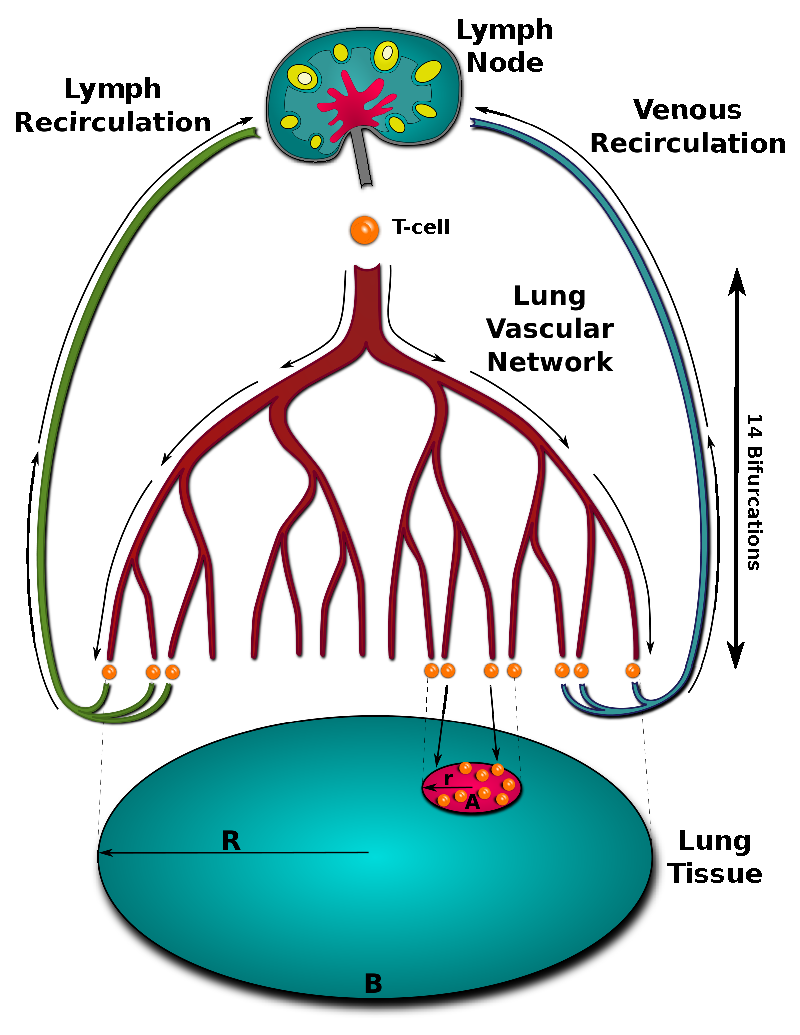
\includegraphics[width=4in]{Figure_1}
\end{center}
\caption{{\bf Model of T cell search.}  Activated T cells originate in the lymph node and enter the bloodstream after which they randomly navigate through 14 vascular bifurcations of the bronchial network.  Upon reaching a capillary, T cells exit into tissue if cytokine signal is present.  In the absence of signal, the T cell recirculates either through the lymph network or through the pulmonary vein back to the top of the network.}
\label{fig:systemchart}
\end{figure}

\begin{figure}[!ht]
\begin{center}
%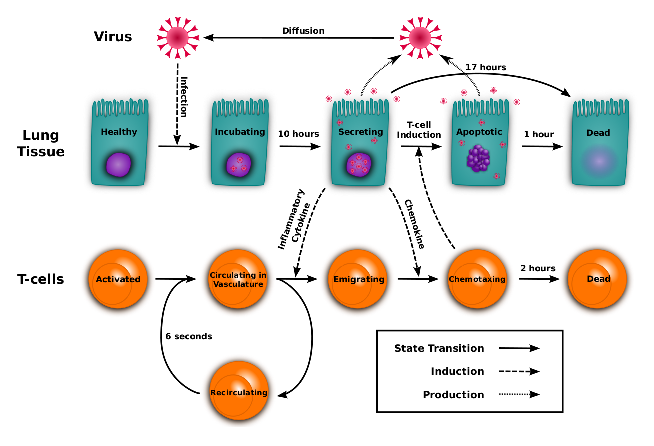
\includegraphics[width=4in]{Figure_2}
\end{center}
\caption{{\bf Visual representation of the model.}  Healthy epithelial cells infected by virus begin secreting virus after the incubation delay.  Activated T cells traverse the bronchial vascular network and may be recruited by inflammatory cytokine.  Chemotaxing T cells climb the chemokine gradient and induce apoptosis in infected cells.  Solid arrows represent a cell state transition from one behavior to another.  Dashed arrows display the mechanism used to induce a transition.  Dotted arrows indicate the production of new virus.}
\label{fig:modelchart}
\end{figure}


\begin{figure}[!ht]
\begin{center}
% 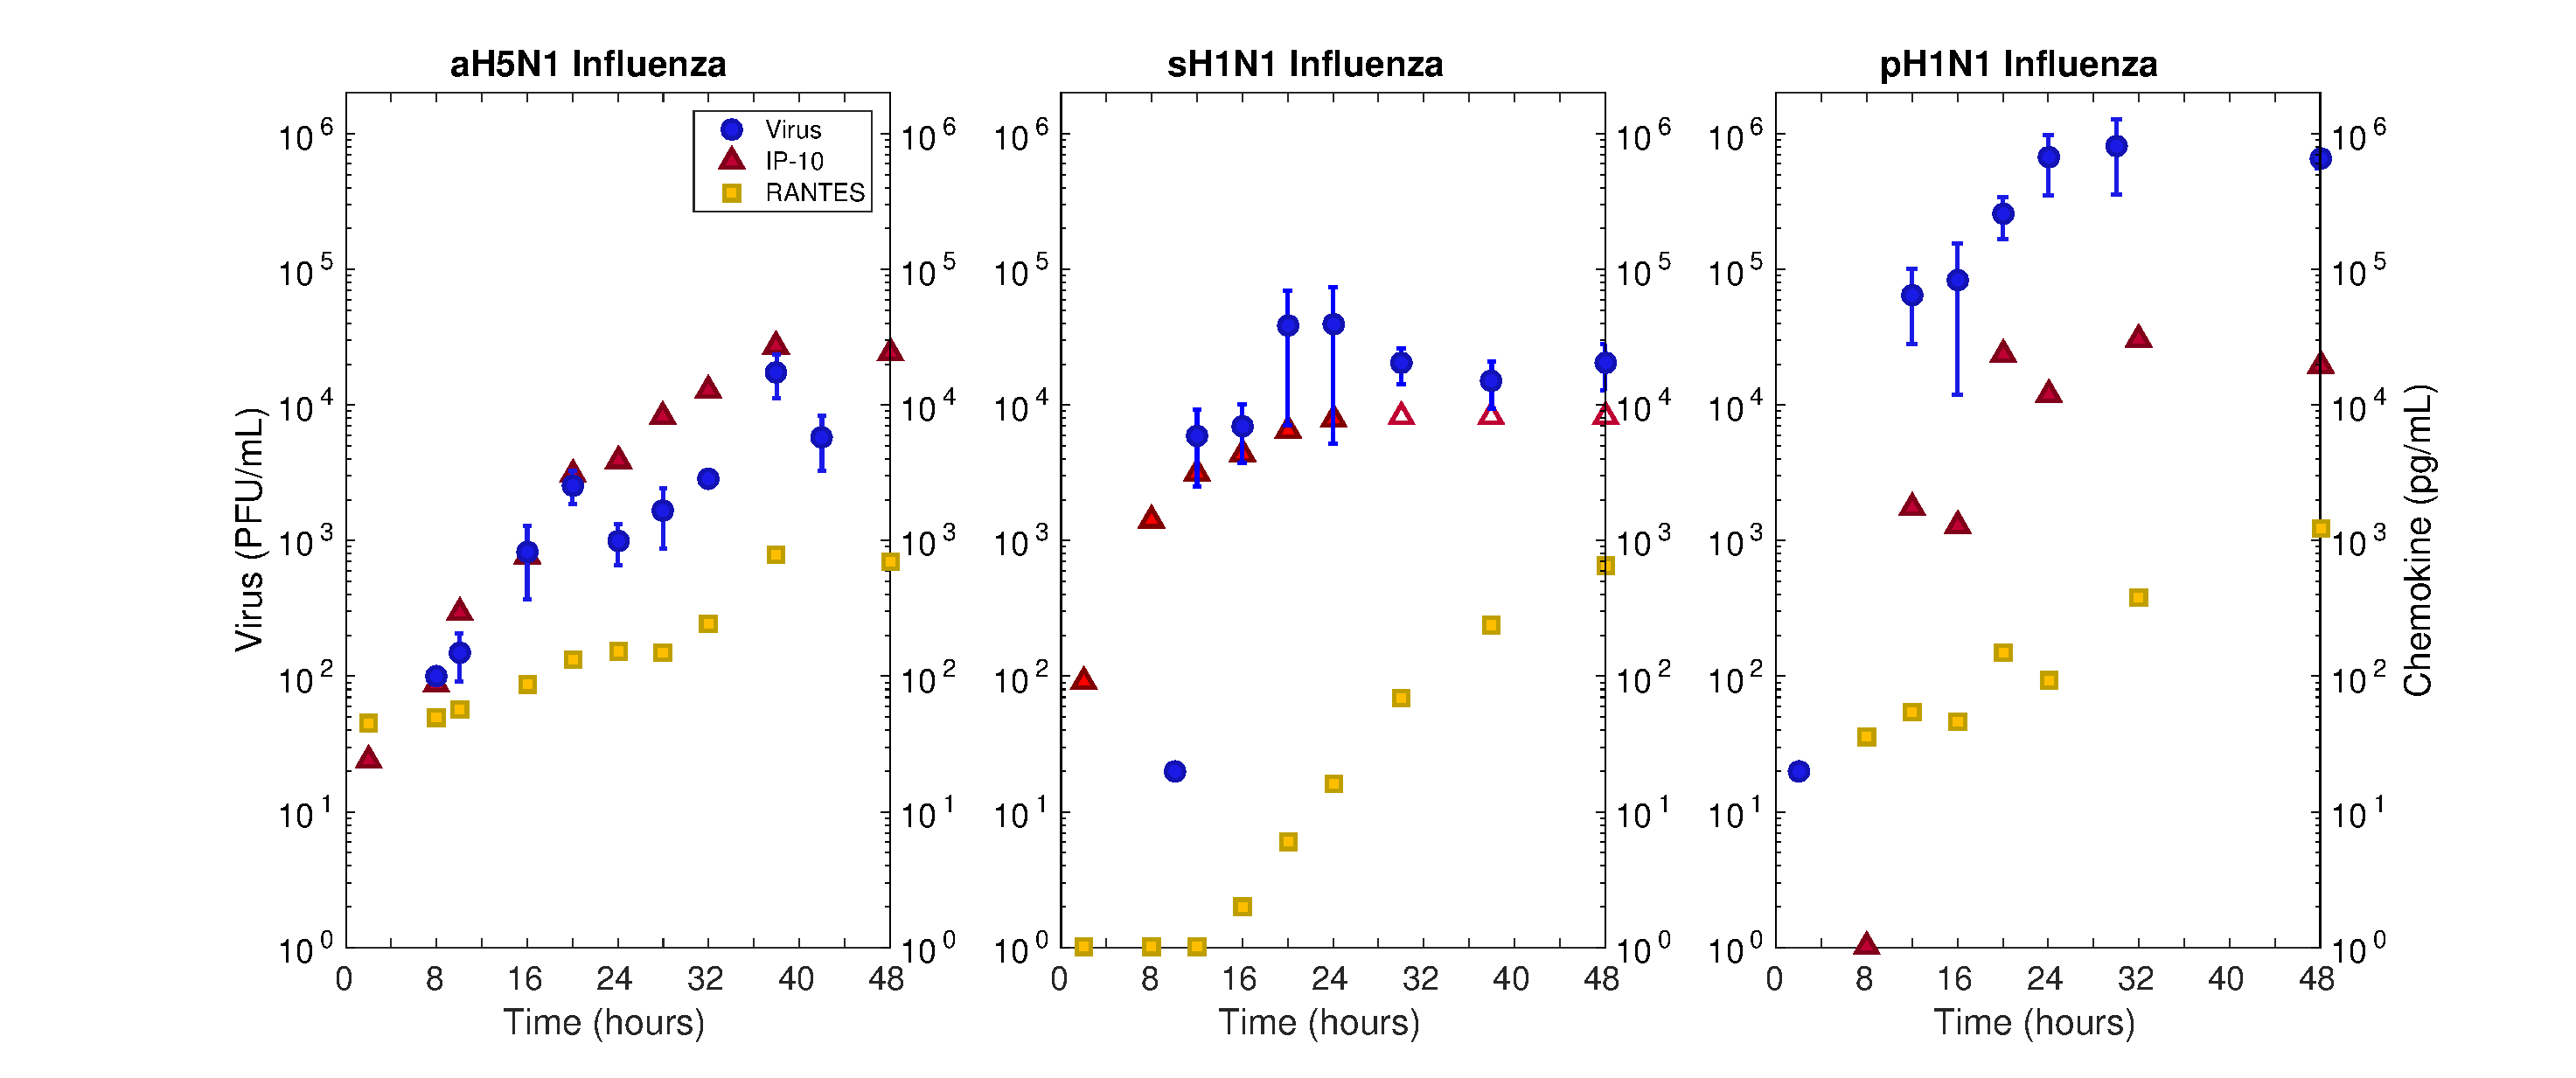
\includegraphics[width=4in]{Figure_3}
 \end{center}
\caption{{\bf Empirical viral and cytokine titers for three strains of influenza: Avian H5N1, Seasonal sH1N1, and Pandemic pH1N1.}  Viral titer (blue circles) is in PFU/mL, and IP-10 (red triangle) and RANTES (green square) are shown in ng/mL.   sH1N1 IP-10 secretion exceeded measurement accuracy above 8500 pg/mL but these three values (empty red triangles) were not included in the model fitting.  Dashed lines show model fits to IP-10 and RANTES data.  Human bronchial epithelial cells were infected at an MOI of 0.01 with one of the three strains of influenza.  Apical fluid for viral secretion and basal media for chemokine secretion was collected at the given time intervals post infection.  Viral culture was performed by a standard plaque assay and chemokine levels were measured using 30 µl aliots for a panel of 17 chemokines and cytokines (not shown).} 
 \label{fig:data}
\end{figure}


\begin{figure}[!ht]
\begin{center}
% 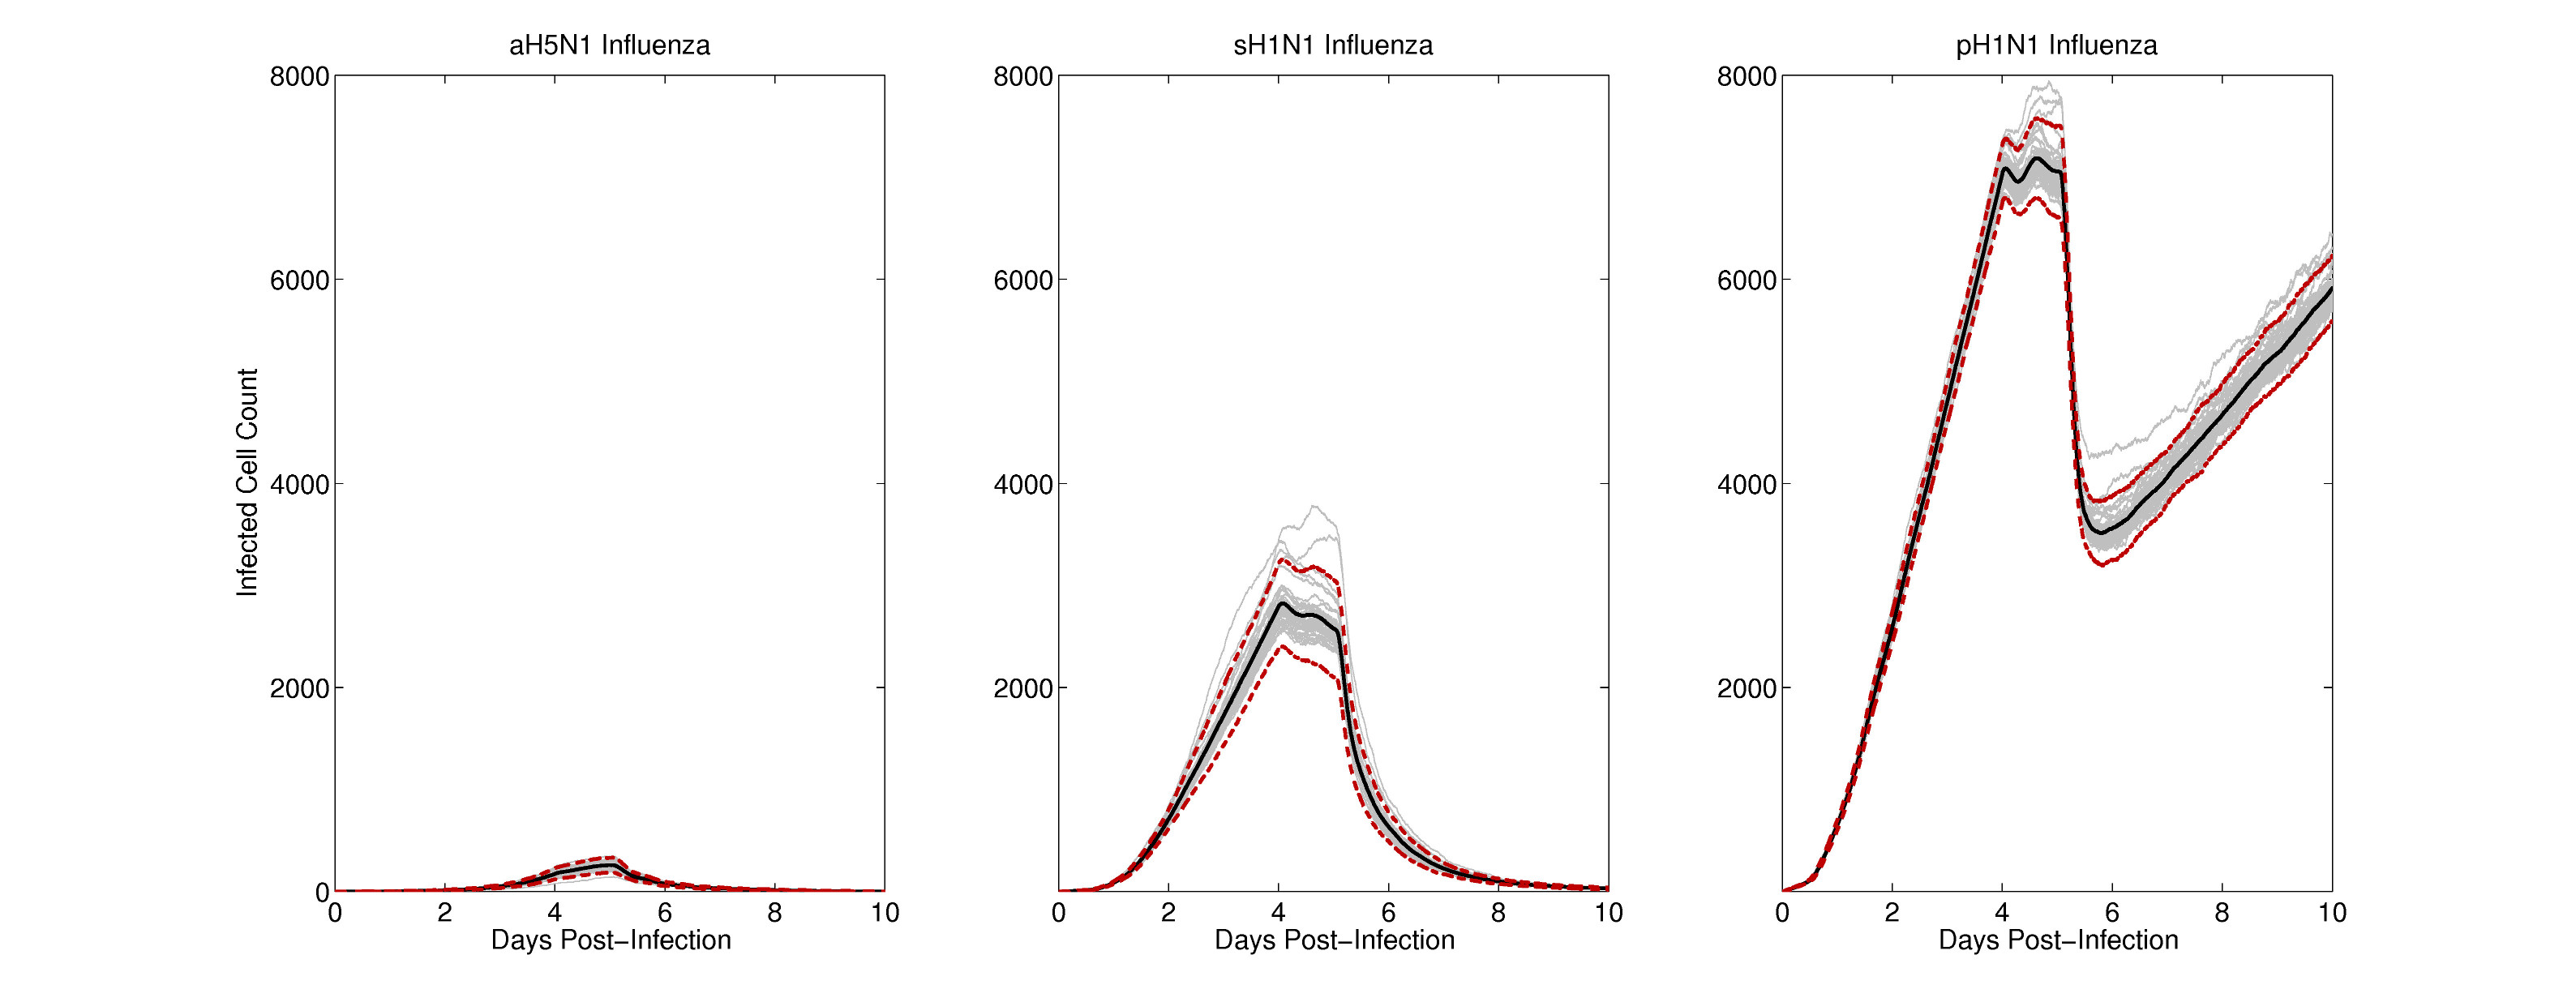
\includegraphics[width=4in]{Figure_4}
 \end{center}
\caption{{\bf Varying T cell sensitivity to chemokine.}  H5N1 model results use RANTES  only, and sH1N1 and pH1N1 use both IP-10 and RANTES. Total number of incubating, secreting and apoptotic cells are plotted for each infection.  The sensitivity value specifies the minimum level of chemokine concentration required for T cells to detect it. } 
 \label{fig:sensitivity}
\end{figure}


\begin{figure}[!ht]
\begin{center}
% 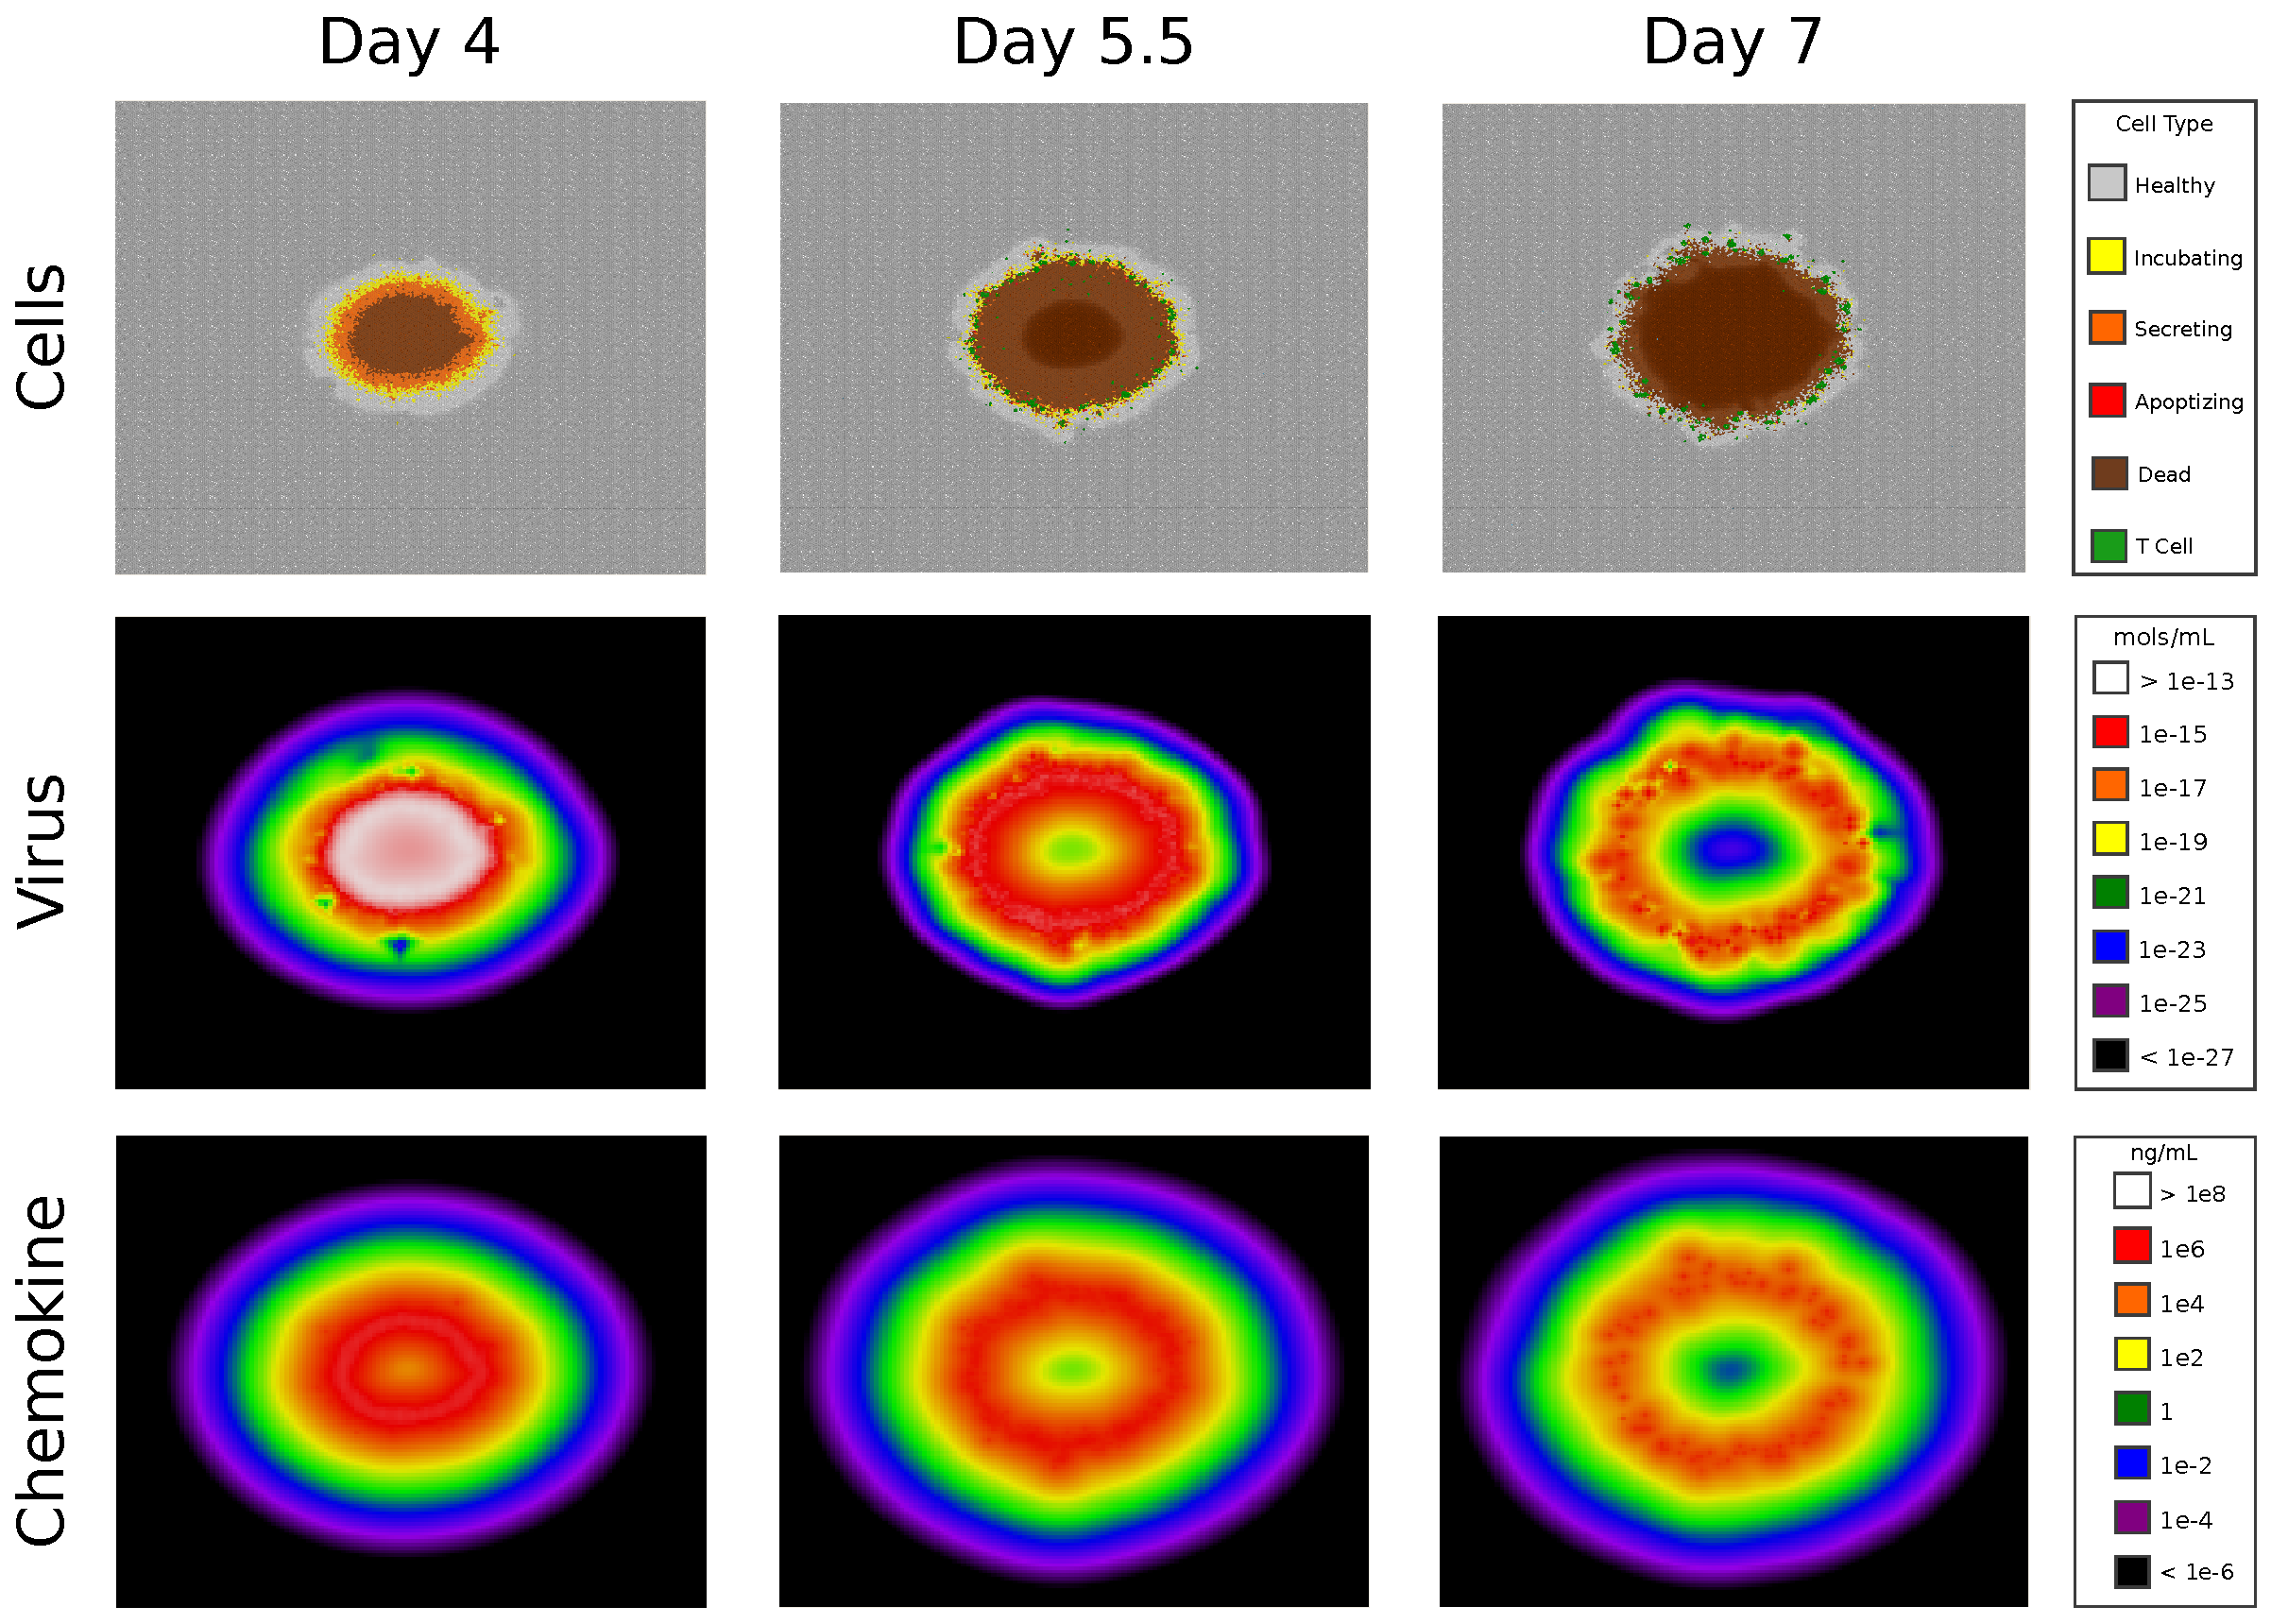
\includegraphics[width=4in]{Figure_5}
 \end{center}
\caption{{\bf Simulated sH1N1 infection.} Screenshots from day 4, day 5.5, and day 7.  The top row shows the spreading focus of infection  through the color coding of individual cells:  healthy cells in uninfected tissue (gray),  virus-incubating cells (yellow), virus-secreting cells (orange), apoptotic cells (red), dead cells (brown), and T cells arriving at day 5 (green).  Free virus and chemokine particles are represented by compartmentalized concentrations of mols/mL and ng/mL.  Individual cell images for days 5.5 and 7 were enhanced (green dots are enlarged) manually to improve T cell visibility.  Thus, individual groups of T cells, which cover only an area of one or two epithelial cells in the model appear larger in the image.  Original images available upon request. } 
 \label{fig:cycells}
\end{figure}


\begin{figure}[!ht]
\begin{center}
% 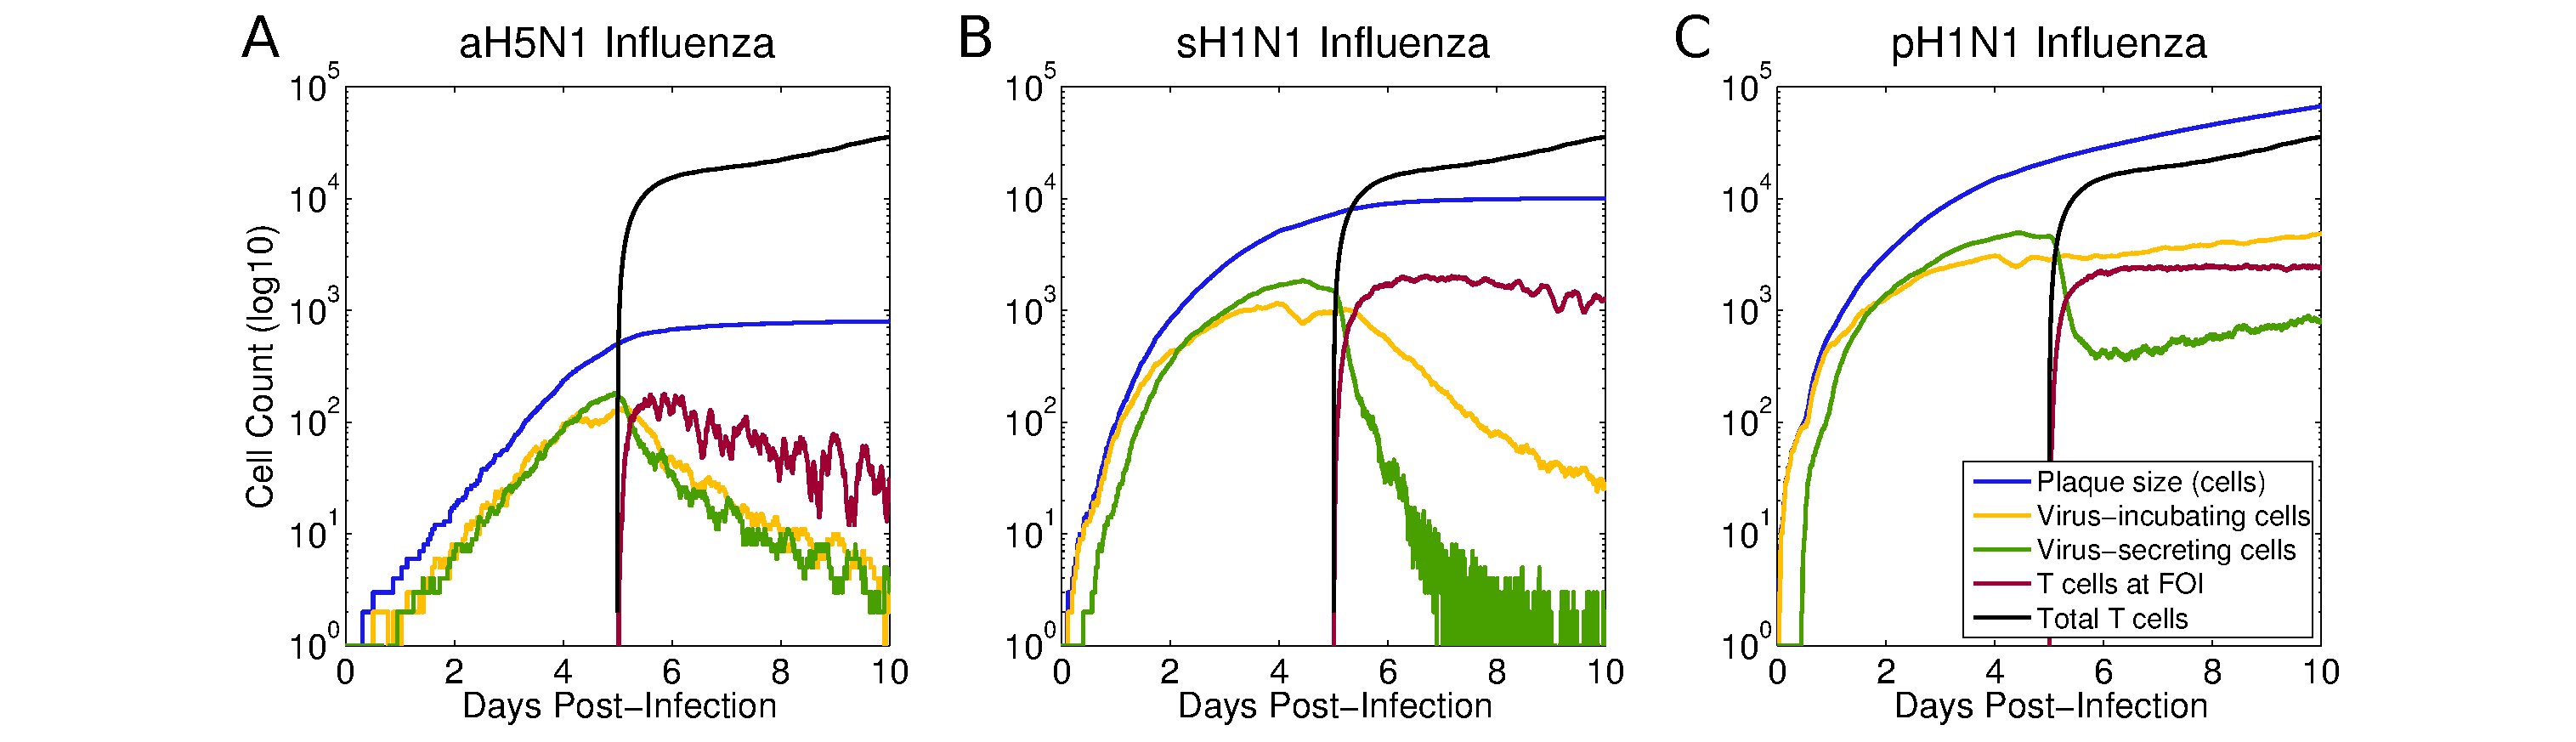
\includegraphics[width=\textwidth]{Figure_6}
 \end{center}
\caption{{\bf Simulated infections of aH5N1, sH1N1, and pH1N1.} Plotted values: total plaque size (blue), number of virus incubating cells (yellow), number of virus secreting cells (green), and T cells (red).  T cells clear secreting and incubating cells in aH5N1, fail to clear incubating cells in sH1N1, and fail to clear either type of infected cell in pH1N1.  The number of expressing cells (green) after day 5 differs markedly among the three strains indicating that the T cells have differing success at controlling the infection.} 
 \label{fig:plaquesize}
\end{figure}

\setcounter{figure}{0}
\renewcommand{\thefigure}{S\arabic{figure}}

\begin{figure}[ht!]
\begin{center}
% 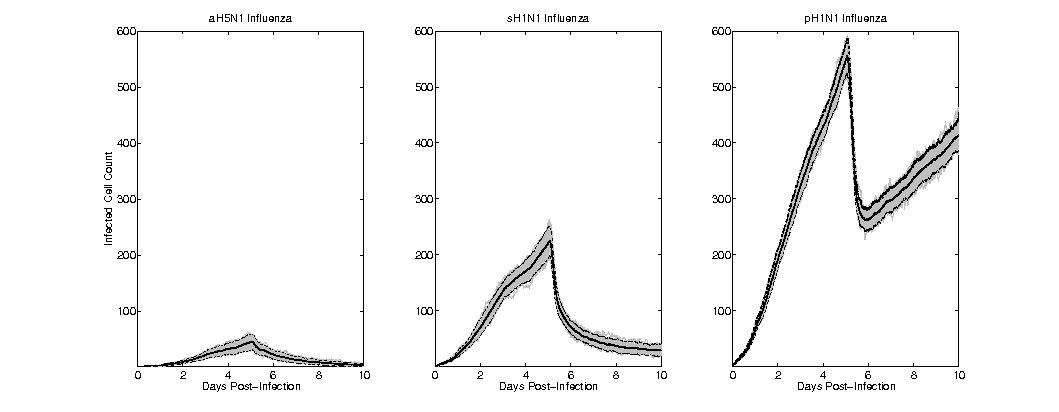
\includegraphics[width=\textwidth]{Figure_S1}
 \end{center}
\caption{Model results: Time series plots of fifty runs of aH5N1 (A), sH1N1 (B), and pH1N1 (C) infections (gray). IP-10 and RANTES were simulated in each run, except for aH5N1, which  produced only RANTES.  Each run was initialized identically for each strain save for the random seed.  The middle line shows the average while the outer lines show the 95\% confidence interval.} 
 \label{fig:variance}
\end{figure}


\begin{figure}[ht!]
\begin{center}
%	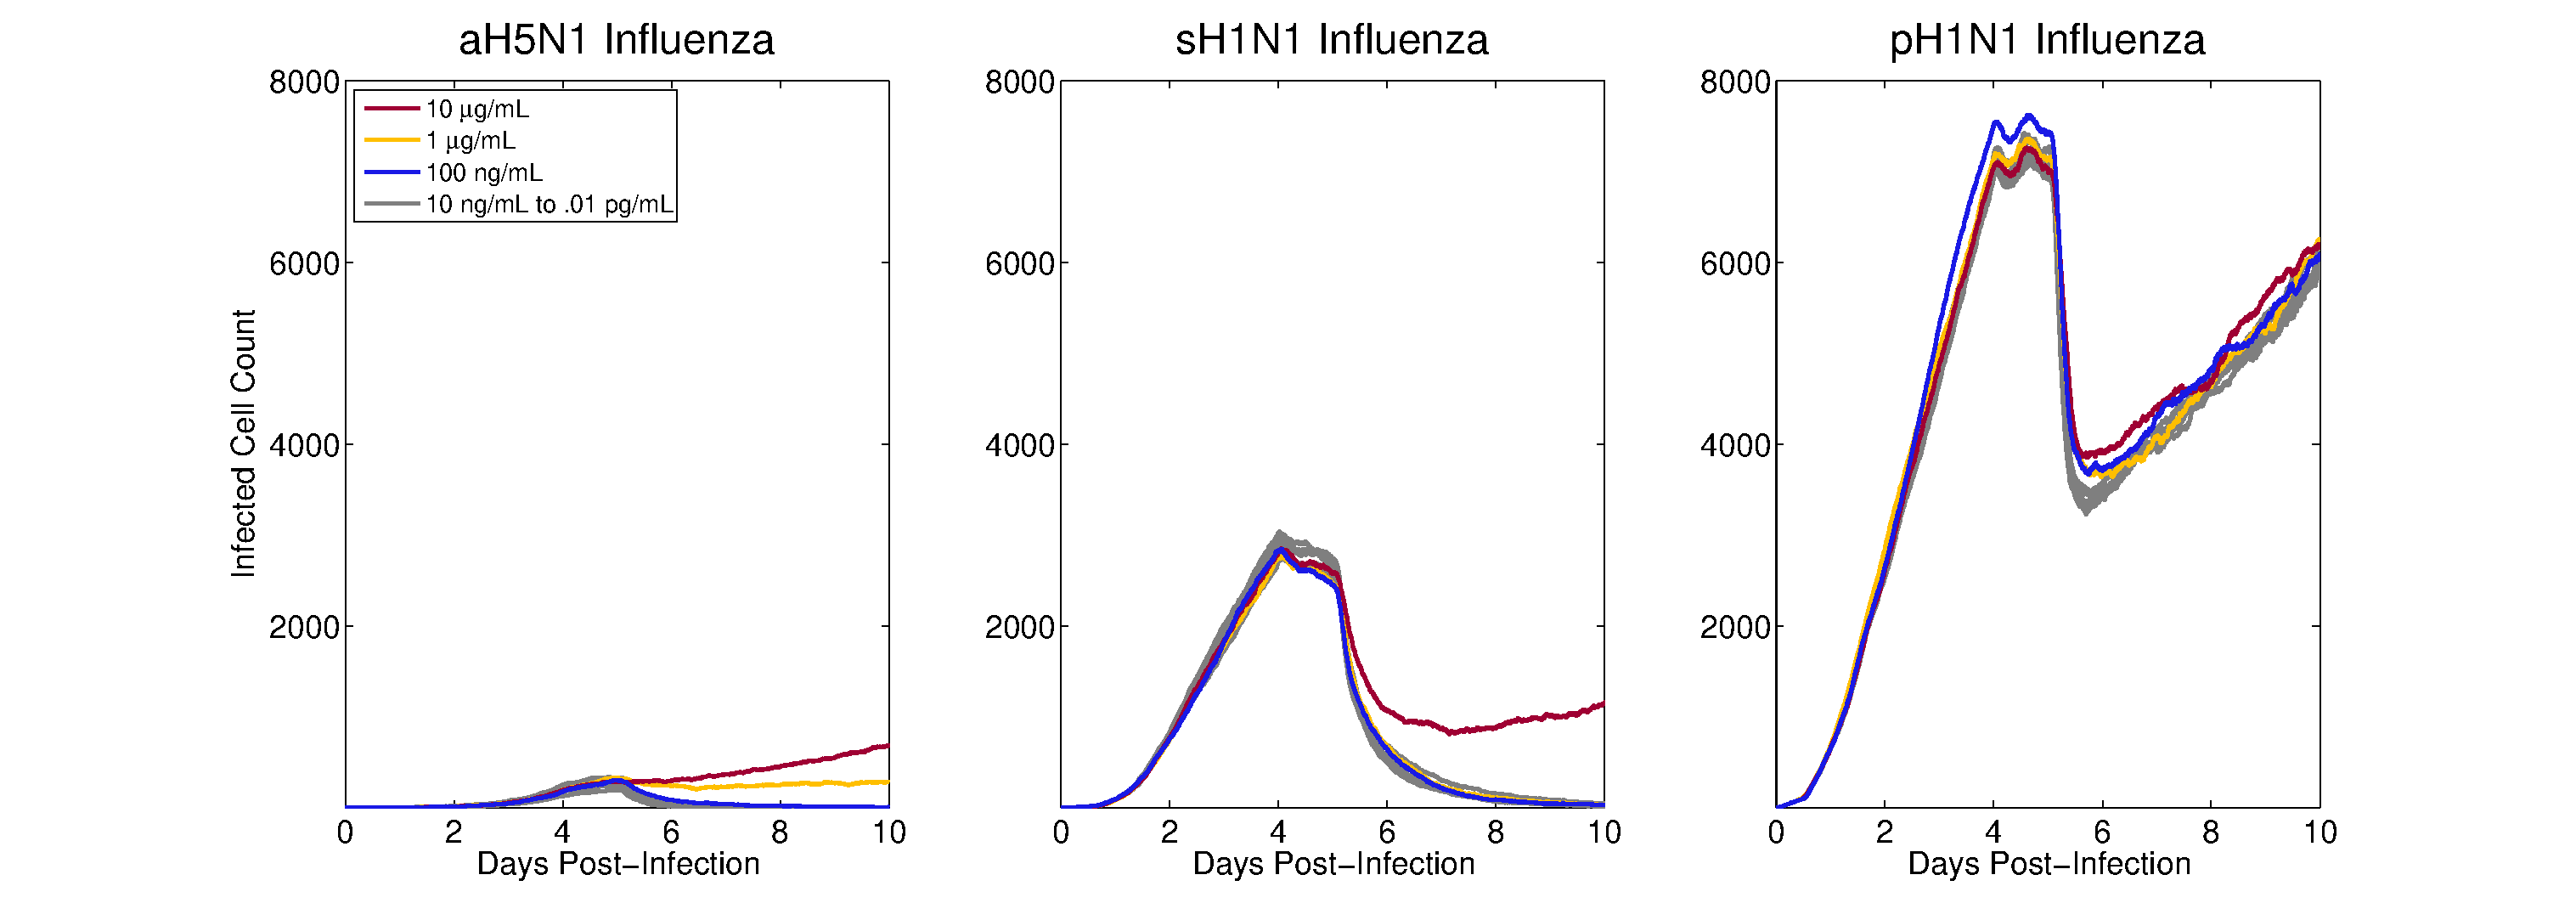
\includegraphics[width=\textwidth]{Figure_S2}
	\caption{Effects of different chemokine combinations.  A) aH5N1 does not stimulate an IP-10 response.  B-C) sH1N1 and pH1N1 show no significant difference between IP-10 alone versus IP-10 and RANTES combined.}
	\label{fig:chemokine}
\end{center}
\end{figure}

\setcounter{figure}{0}
\renewcommand{\figurename}{Video}

\begin{figure}[ht!]
\caption{The first of three overlaid videos of a representative seasonal H1N1 infection.  This video spans the 10 day infection and shows the cells as they transition from healthy to infected to dead.  T cells show half way through the simulation.  Healthy cells are gray, virus-incubating cells are yellow, virus-secreting cells are orange, apoptotic cells are red, and T cells are green.} 
 \label{video:cell_view}
\end{figure}

\begin{figure}[ht!]
\caption{The second of three overlaid videos of a representative seasonal H1N1 infection.  This video spans the 10 day infection and shows the virus concentration.  Notice the volatility when T cells arrive halfway through the simulation.  Virus concentration ranges from 1e-13 mols/mL (white) to 1e-27 mols/mL (black).  Refer to Figure 5 for the detailed legend. } 
 \label{video:virus_view}
\end{figure}

\begin{figure}[ht!]
\caption{The third of three overlaid videos of a representative seasonal H1N1 infection.  This video spans the 10 day infection and shows the chemokine concentration.  Notice the volatility when T cells arrive halfway through the simulation.  Chemokine concentration ranges from 1e8 ng/mL (white) to 1e-6 ng/mL (black).  Refer to Figure 5 for the detailed legend. } 
 \label{video:chemokine_view}
\end{figure}

\begin{figure}[ht!]
\caption{A closer look at the 2009 pandemic simulation.  This video shows the infection from day 6 to day 7 with each frame spanning 100 simulated seconds.  Healthy cells are gray, virus-incubating cells are yellow, virus-secreting cells are orange, apoptotic cells are red, and T cells are green.  Note the high proportion of virus-secreting cells (orange) early on.  As time passes, secreting cells are gradually contained to the point where they become very sparse.  T cell clumping often prevents the T cells from quick discovery of new secreting cells.}
\end{figure}

\pagebreak

\section*{Tables}
%\begin{table}[!ht]
%\caption{
%\bf{Table title}}
%\begin{tabular}{|c|c|c|}
%table information
%\end{tabular}
%\begin{flushleft}Table caption
%\end{flushleft}
%\label{tab:label}
% \end{table}

\begin{table}
\begin{center}
\begin{tabular}{|  l  l  l  |}
  \hline
  Population & Description & Initial Value\\
  \hline
  $T$ & Healthy target epithelial cells & 1,000,000 \\
  $I_1$ & Virus-incubating cells & 0 \\
  $I_2$ & Virus-secreting cells & 0 \\
  $V$ & Free virus particles & 10,000 \\
  $F$ & Interferon quantity & 0 \\
  $C$ & Chemokine quantity (ng/mL) & 0 \\
  \hline
  \hline
  Parameter & Description & Value \\
  \hline
  $\beta$ & Viral infection rates &  \\
    & \hspace{2em} Avian & 5.3e-7 (PFU$\cdot$h)$^{-1}$ \\
    & \hspace{2em} Seasonal & 6.1e-7 (PFU$\cdot$h)$^{-1}$ \\
    & \hspace{2em} Pandemic &  2.7e-6 (PFU$\cdot$h)$^{-1}$\\
  $p$ & Viral production rates & \\
    & \hspace{2em} Avian & 0.20 (PFU/h) \\
    & \hspace{2em} Seasonal & 1.4 (PFU/h) \\
    & \hspace{2em} Pandemic & 18.3 (PFU/h) \\
  $e$ & Interferon strengths & \\
    & \hspace{2em} Avian & 1.0e-8 \\
    & \hspace{2em} Seasonal & 1.6e-6 \\
    & \hspace{2em} Pandemic & 3.4e-3 \\
  $\tau_2$ & Interferon production delays &  \\
    & \hspace{2em} Avian & 21.5 (h) \\
    & \hspace{2em} Seasonal & 23.6 (h) \\
    & \hspace{2em} Pandemic & 21.0 (h) \\
  $\delta$ & Virus-secreting cell decay rate & 0.6 (h$^{-1}$) \\
  $d$ & Chemokine decay rate & 1.386 (h$^{-1}$) \\
  $\tau_1$ & Viral incubation time & 10 (h) \\
  $\tau_3$ & Chemokine production delays & \\
    & \hspace{2em} IP-10 & 8 (h)\\
    & \hspace{2em} RANTES & 16 (h)\\
  \hline
\end{tabular}
\caption{All parameters and populations are taken from \cite{Mitchell2011} except for $C$, $d$, and $\tau_3$.  The value chosen for $d$ corresponds to a 30 minute half-life and values for $\tau_3$ were take from the observed chemokine data (Fig.~\ref{fig:data}).  Interferon ($F$) is an abstracted unitless quantity and thus $e$ is a unitless multiplier.}
\label{tab:dde}
\end{center}
\end{table}



\begin{table}
\begin{center}
\begin{tabular}{| l l l |}
  \hline                        
  Referenced Parameters & Value & Source \\
  \hline
  Viral Diffusion in Airway & .0318 $\mu$m$^2$/s & \cite{Beauchemin2006} \\
  Viral Decay in Airway &  1/day & \cite{Lee2009} \\
  Chemokine Diffusion Rate & .318 $\mu$m$^2$/s & \cite{Beauchemin2006} \\
  Incubation Time &  10 hours & \cite{Mitchell2011} \\
  T cell Production Rate & 777/hour & \cite{Miao2010} \\ 
  Blood Circulation Time & 6 minutes & \cite{Banerjee2010b} \\
  Search Time In Chemokine-Free Tissue & 10 minutes & \cite{Banerjee2010b} \\
  T Cell Sensitivity to Chemokine & 10 ng/mL & \cite{Gao2003} \\
  Onset of ATC$^\ddagger$ Lymph Node Exit & 5 days & \cite{Banerjee2011} \\
  \hline
  \hline                        
  Estimated Parameters & Value & Footnote \\
  \hline
  Chemokine Decay Rate &  $3.8508\cdot10^{-4}$/s & 1\\
  Infection Sensitivity Rate &  2 hour/virion &  2 \\
  Expression Time &  16.7 hours & \cite{Mitchell2011}$^3$ \\
  T Cell Expected Kill Time & 10 min & 4 \\
  Apoptosis Time & 60 minutes & \cite{Ganusov2008}$^5$ \\
  Epithelial Cell Radius & 25 $\mu$m & 6 \\
  T Cell Age (at FOI$^\ast$) & 2 hours & 7 \\
  T Cell Age (in Blood) & 3 days & 7 \\
  T Cell Speed (Search) & 30 $\mu$m/s & \cite{Miller2003}$^8$ \\
  T Cell Speed (Chemotaxis) & 3 $\mu$m/s & \cite{Miller2003}$^8$ \\
  IgM Strength & Viral decay of 3/day & 9 \\
  \hline  
\end{tabular}
\caption{Values are taken from literature if possible, otherwise values are estimated as follows.  1) Corresponds to a 30 minute half-life.  2) Epithelial cells are infected at a probabilistic rate such that the expected time for infection in the presence of a single virion is 2 hours.  This scales linearly with the number of virions in the cell's vicinity.  3) Chosen as a plausible median time (1,000 minutes) between 6 hours and 24 hours.  4) T cells induce apoptosis in nearby virus-secreting epithelial cells at a probabilistic rate such that the expected time to induce apoptosis is 10 minutes.  This rate does not scale with T cell numbers.  5) Calculated for low T cell densities.  6) The mean surface area of the epithelial cell available for virus contact and entry includes cilia and the radius is estimated to be 25 microns. 7) Chosen to be at the lower end of biologically plausible values because increased T cell counts are shown not to affect the model behavior.  8) The values were selected to be an order of magnitude faster than those calculated for inside the lymph node.  9) IgM presence is abstracted by increasing viral decay by a factor of three. $^\ddagger$Activated T Cell.  $^\ast$Focus of Infection.}
\label{tab:parameters}
\end{center}
\end{table}



\begin{table}
\centering
\begin{tabular}{ | r | c | c | c | }
  \hline                        
  \multicolumn{1}{|c|}{\multirow{2}{*}{Strain}} & IP-10 Production & RANTES Production & Viral Production \\
   & \footnotesize{$(pg/s\cdot cell)$}  & \footnotesize{$(pg/s\cdot cell)$} &  \footnotesize{$(PFU/s\cdot cell)$} \\
  \hline
  \multirow{2}{*}{Avian H5N1} & 2.0e-4 &  1.3e-5 & 5.4e-5 \\
   &  \footnotesize{8.4e-5 --- 4.2e-4} & \footnotesize{7.9e-6 --- 1.9e-5} & \footnotesize{4.4e-5 --- 3.7e-4}\\ 
   \hline
  \multirow{2}{*}{Seasonal H1N1} & 1.8e-4 &  8.9e-7 & 3.8e-4 \\
   & \footnotesize{1.2e-4 --- 3.0e-4} & \footnotesize{4.8e-7 --- 1.6e-6} & \footnotesize{2.8e-4 --- 1.5e-3}\\
   \hline
  \multirow{2}{*}{Pandemic H1N1} & 8.7e-5 &  4.3e-6 & 5.1e-3 \\
   & \footnotesize{1.7e-5 --- 7.1e-4} & \footnotesize{5.0e-7 --- 3.5e-5} & \footnotesize{2.8e-3 --- 5.3e-3} \\
  \hline
\end{tabular}
\caption{Strain-specific model parameters.  Small text values show 95\% confidence intervals resulting from 1,000 bootstrapping runs for each parameter \cite{Wu1986}.  Viral production values are taken from \cite{Mitchell2011}.}
\label{tab:strains}
\end{table}


\end{document}

